\documentclass[norsk,a4paper,12pt]{article} 
\usepackage[norsk]{babel} 
\usepackage[T1]{fontenc} %for å bruke æøå 
\usepackage[utf8x]{inputenc} 
\usepackage{graphicx} %for å inkludere grafikk 
\usepackage{verbatim} %for å inkludere filer med tegn LaTeX ikke liker 
\usepackage{amsfonts} 
\usepackage{amsmath} 
\usepackage{amssymb} 
%\usepackage{savesym} 
%\savesymbol{square} 
\bibliographystyle{plain} 
\usepackage{float} 
%\usepackage{SIunits} 
\usepackage{textcomp} 
\usepackage{parskip} 
\usepackage{array} 
%\usepackage[framed]{mcode} 
\usepackage[margin=2.3cm]{caption}
\usepackage{listings}

\begin{document}

\title{AST5220 Cosmology II: Milestone 1}
\author{Peder Forfang}
\maketitle



\section{The background evolution of the Universe}
The Cosmic Microwave Background (CMB) anisotropies is an important source of information on the history of the Universe and since first discovered has been a large research field in cosmology. This report is the first part of a larger project concerning calculation of the CMB spectrum. Here we will concern ourselves with calculation of the expansion history of the Universe and the uniform background densities of the various matter and energy components from recombination until today. The report includes a description of the computed quantities as well as plots of $H(z)$, $H(x)$, $\eta (x)$ and one plot of $\Omega_b(x)$, $\Omega_m(x)$, $\Omega_r(x)$ and $\Omega_{\Lambda}(x)$ together. For the sake of simplicity we will neglect the neutrino densities $\Omega_{\nu}$. The source code of the numerical calculations done in FORTRAN will be attached as well.

The background geometry is given by the Friedmann-Robertson-Walker metric (assuming flat space, $k=0$):

\begin{equation}
 ds^2 = -c^2dt^2 + a^2(t)(dr^2 + r^2(d\theta^2 + sin^2\theta d\phi^2) 
\end{equation}

\begin{equation}
 = a^2(t)(-d^2\eta + dr^2 + r^2(d\theta^2 + sin^2\theta d\phi^2))
\end{equation}

The quantity $\eta$ is the conformal time describing the distance light may have travelled since Big Bang. Since the speed of light is the absolute speed limit, $\eta$ may be thought of as the ``horizon'' of the Universe. In our case it is convenient to use the logarithmic of the scale factor, as we are dealing with such large time scales. Thus we introduce $x = log a$ as our time variable. Another important quantity we need to introduce is the redshift $z$, defined as:

\begin{equation}
 \frac{a_0}{a(t)} = 1 + z
\end{equation}

where $a_0 = 1$ is the scale factor today. The expansion of the Universe is given by the Friedmann equation

\begin{equation}
 H \equiv \frac{1}{a}\frac{da}{dt} = H_0\sqrt{(\Omega_b + \Omega_m)a^{-3} + \Omega_ra^{-4} + \Omega_{\Lambda})}
\end{equation}

Here $H$ is the Hubble parameter, in which $H_0$ is the current value and $\Omega_x$ the densities of their respected quantities (baryonic matter(b), dark matter(m), radiation(r) and dark energy($\Lambda$)) relative to the critical density $\rho_c$

\begin{equation}
 \Omega_x = \frac{\rho_x}{\rho_c}
\end{equation}

\begin{equation}
 \rho_c = \frac{3H^2}{8\pi G}
\end{equation}

The key to this task is to look at how the conformal time evolves. To do this we need a computable expression for  $\eta$. We have that

\begin{equation}
 \frac{d\eta}{dt} = \frac{c}{a}
\end{equation}

\begin{equation}
 \Rightarrow \frac{d\eta}{dt} = \frac{d\eta}{da}\frac{da}{dt} = \frac{d\eta}{da}aH
\end{equation}

\begin{equation}
 \Rightarrow \frac{d\eta}{da} = \frac{c}{a^2H} = \frac{c}{aH_p}
\end{equation}


where $H_p \equiv aH$. We will use this differential equation numerically by plugging it into an ordinary differential solver. The conformal time thus takes the form

\begin{equation}
 \eta(a) = \int_0^a \frac{da}{a H_p(a)} 
\end{equation}


from which we can extract initial values. As $a\rightarrow 0$ we note that $aH_p(a) \rightarrow H_0\sqrt{\Omega_r}$. Thus our initial value is  

\begin{equation}
 \eta(a\rightarrow 0) = \frac{a}{H_0\sqrt{\Omega_r}}
\end{equation}

and $\eta(x) = \eta(a=e^x)$. Setting this up numerically we define our time frame to go from $ x = ln(1\times10^{-10})$ to $x = 0$, which is our time today. The following figures shows how $H(x), H(z), \eta(x) $ and the various densities evolve throughout the expansion. 



\begin{figure}[H] 
\begin{center} 
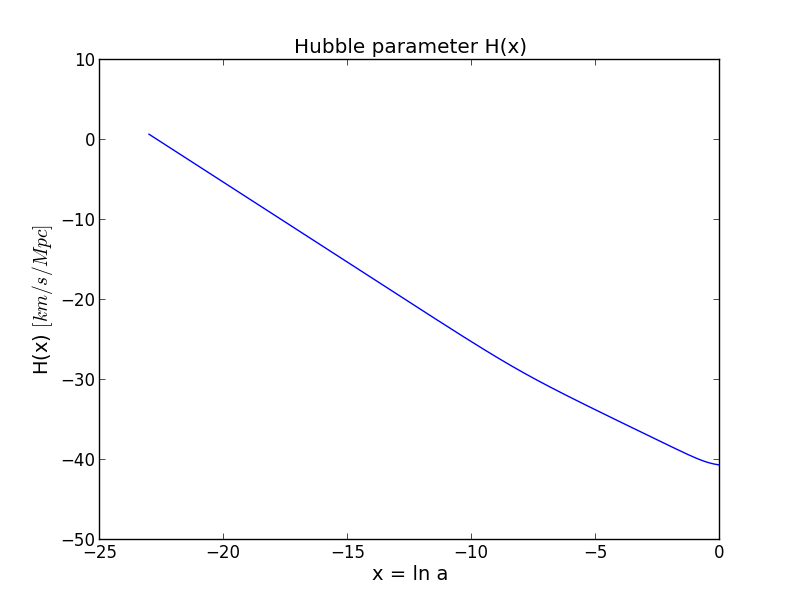
\includegraphics[scale=0.5]{hubblex.png} 
 

\caption{The Hubble parameter as function of x. Present time is at $x = ln a = 0$. (Note to reader: I could not quite figure out the trouble with my y-axis in this plot).} 
\end{center} 
\end{figure}


\begin{figure}[H] 
\begin{center} 
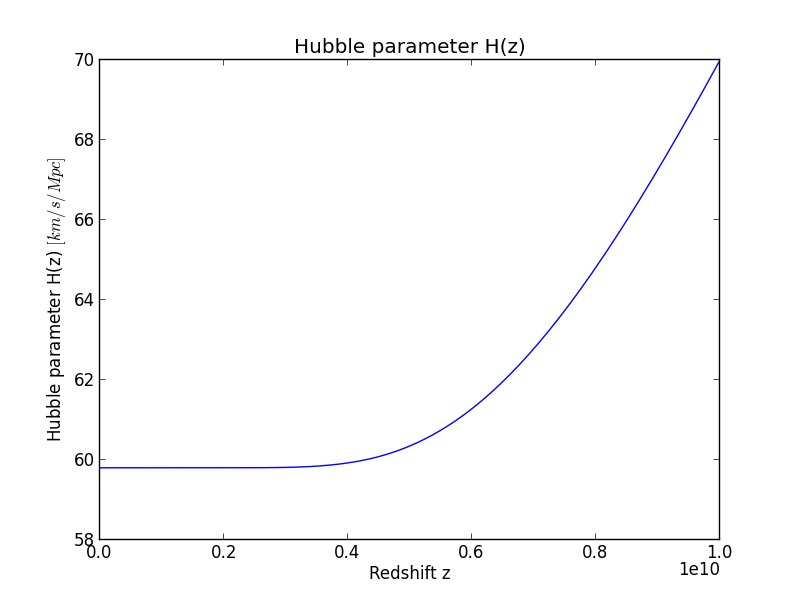
\includegraphics[scale=0.5]{hubblez.png} 
 

\caption{The Hubble parameter as a function of z. The present is at far left, hence the increasing redshift. The hubble parameter describes the expansion of the Universe. Today the actual value is about $H_0 = 67,8$ (km/s)/Mpc. Alas this estimation is a little off.} 
\end{center} 
\end{figure}


\begin{figure}[H] 
\begin{center} 
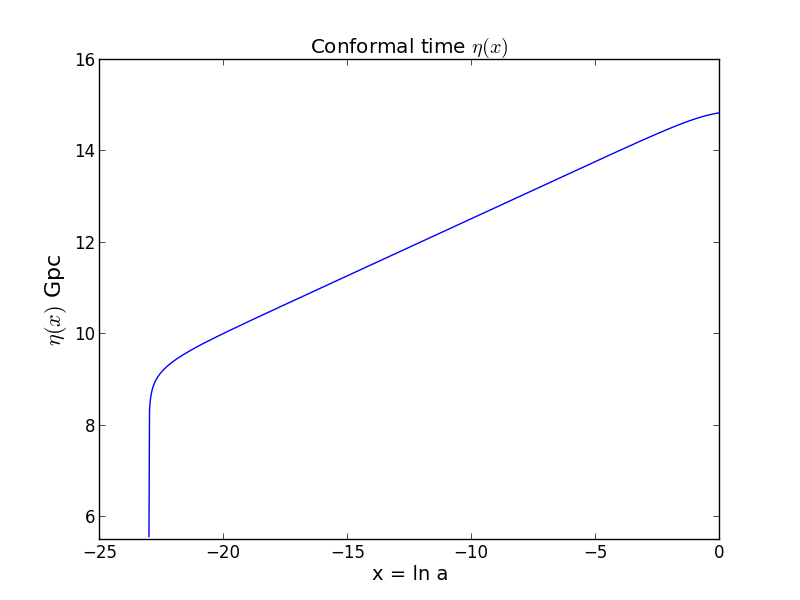
\includegraphics[scale=0.5]{eta.png} 
 

\caption{This plot shows the conformal time $\eta$ as a function of x. As the picture shows, $\eta$ grows vertically in the beginning. It indicates the very fast expansion believed to take place in primordial times. From there it grows more linear towards today. The present value of the conformal time can be found at x = 0. The real value is about 14.4 Gpc.} 
\end{center} 
\end{figure}




\begin{figure}[H] 
\begin{center} 
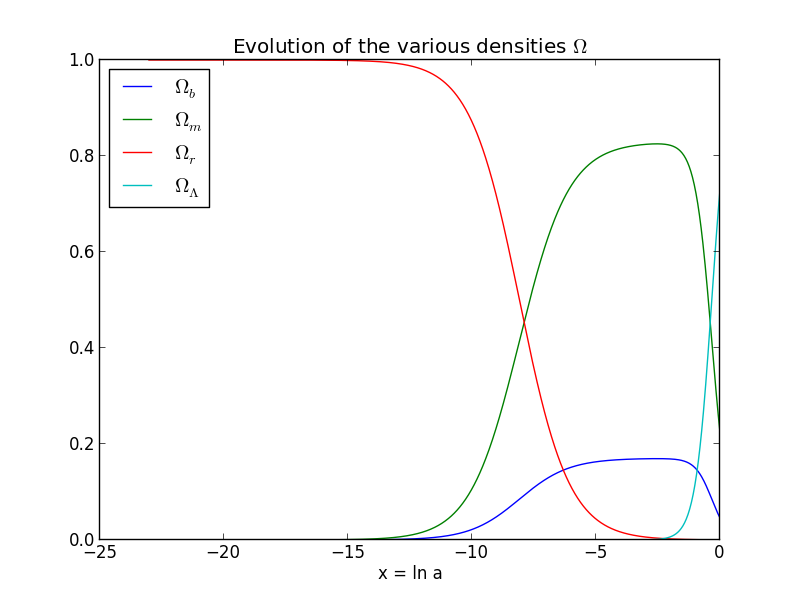
\includegraphics[scale=0.5]{omegaplot.png} 
 

\caption{The densities of baryons(b), dark matter(m), radiation(r) and dark energy($\Lambda$). The picture is interesting as it displays the various epochs of our history in a simple way. The radiation had total domination early on, until the Universe cooled sufficiently to allow matter to settle. The point where the red line (radiation line) cross the green line (dark matter line) marks the point of matter-radiation equality. Recombination is a bit more difficult to pinpoint at this stage. Recall that $1+z = 1/a(t)$ and that recombination happened about z = 1100. Here this would correspond to $x\approx-3$, close to where $\Omega_r$ reaches its minimum.} 
\end{center} 
\end{figure}










\end{document}

